\documentclass[journal]{IEEEtran}

\usepackage{amsmath,amssymb,amsfonts}
\usepackage{graphicx}
\usepackage{textcomp}
\usepackage{xcolor}
\usepackage{booktabs}
\usepackage{multirow}
\usepackage{url}
\usepackage{hyperref}
\usepackage{balance}

\begin{document}

\title{Higher Rank, More Hallucination? How LoRA Capacity and Data Quality Interact to Control Label Compliance in Fine-Tuned LLMs}

\author{
\IEEEauthorblockN{Nutthakorn Chalaemwongwan}
\IEEEauthorblockA{Department of Computer Engineering, KOSEN-KMITL\\
King Mongkut's Institute of Technology Ladkrabang\\
Bangkok, Thailand\\
nutthakorn.ch@kmitl.ac.th}
}

\maketitle

\begin{abstract}
LoRA rank selection is widely treated as an accuracy hyperparameter, yet its effect on label compliance remains unexplored. We present a controlled ablation of Qwen3.5-9B fine-tuned for SOC alert classification across ranks \{16, 32, 64, 128\}, learning rates \{$1\times10^{-4}$, $2\times10^{-4}$, $5\times10^{-4}$\}, and two data quality conditions (clean zero-overlap splits vs.\ noisy leaked data). Our central finding is that \textbf{data quality dominates all hyperparameter effects}: on clean data, ranks 16 and 32 achieve perfect strict F1 (100\%), while the same configurations degrade to 98.4\% and 79.4\% on noisy data. A previously reported rank-32 anomaly (F1=36.0\%) was entirely a data leakage artifact---on clean data, rank 32 equals rank 16 at 100\%. Learning rate effects are parallel: $1\times10^{-4}$ achieves perfect compliance on clean data while $5\times10^{-4}$ degrades to 75.4\%. We formalize a \emph{rank-compliance tradeoff} (Definition~1): lower ranks limit the dimensionality of pre-training knowledge that can surface, while higher ranks provide more pathways for label vocabulary hallucination. However, very high rank (128) shows U-shaped recovery on noisy data (93.5\%), suggesting sufficient capacity can also help override pre-training. Our results establish that hyperparameter ablation on leaked data produces fundamentally misleading conclusions, and we recommend data integrity verification as a prerequisite to any PEFT study.
\end{abstract}

\begin{IEEEkeywords}
LoRA, rank ablation, label compliance, parameter-efficient fine-tuning, data leakage, QLoRA
\end{IEEEkeywords}

%% ===== INTRODUCTION =====
\section{Introduction}

Low-Rank Adaptation (LoRA)~\cite{hu2022} has become the dominant parameter-efficient fine-tuning (PEFT) method, with rank selection typically guided by accuracy-compute tradeoffs. A common heuristic is ``start with rank 8--16, increase if accuracy is insufficient.'' However, this guidance considers only a single evaluation dimension: accuracy or loss.

We identify a second, critical dimension---\emph{label compliance}---that exhibits qualitatively different behavior with respect to rank. Label compliance measures whether a model outputs the exact label string specified by the task schema, rather than a semantically equivalent alternative. In production systems (SOC automation, medical coding, legal categorization), exact label matches are required for downstream integration---a prediction of ``Port Scanning'' when the schema specifies ``Reconnaissance'' causes pipeline failures regardless of semantic correctness.

Our investigation reveals three unexpected findings:
\begin{enumerate}
\item \textbf{Lower ranks achieve better compliance on clean data}. Ranks 16 and 32 achieve perfect strict F1 (100\%), while rank 64 drops to 83.6\% due to knowledge activation.
\item \textbf{Data quality dominates rank selection}. Every rank performs substantially better on clean data. The improvement ranges from +1.6 points (rank 16) to +27.9 points (rank 64).
\item \textbf{Previously reported anomalies are leakage artifacts}. A rank-32 anomaly (F1=36.0\%) disappears entirely on clean data (F1=100\%), demonstrating that data leakage can produce \emph{directionally wrong} hyperparameter conclusions.
\end{enumerate}

These findings establish that data integrity verification is a \emph{prerequisite}---not an afterthought---for any PEFT hyperparameter study. Our companion studies identified label hallucination~\cite{p3}, non-monotonic scaling~\cite{p6}, cost efficiency~\cite{p7}, multi-task regularization~\cite{p15}, architecture effects~\cite{p21}, task entropy~\cite{p8}, cascade routing~\cite{p5}, and evaluation methodology~\cite{p19}. Ferrag et~al.~\cite{ferrag2024} surveyed LLMs for cybersecurity; Ouyang et~al.~\cite{ouyang2022} established RLHF as a baseline alignment technique. This paper reveals that \emph{LoRA rank} interacts with both data quality and pre-training knowledge to control hallucination.

Our contributions:
\begin{enumerate}
\item A $4 \times 3 \times 2 = 24$-configuration grid ablation studying rank $\times$ learning rate $\times$ data quality on label compliance.
\item The \textbf{rank-compliance tradeoff} (Definition~1): a formalized non-monotonic relationship between LoRA rank and label compliance.
\item Demonstration that \textbf{data quality dominates} rank by up to 27.9 points, establishing a clear priority: fix data first.
\item A \textbf{leakage case study}: rank-32 anomaly (F1=36.0\%) is 100\% attributable to data leakage; true performance is 100\%.
\item Evidence for \textbf{U-shaped rank recovery}: very high rank (128) partially recovers from knowledge activation.
\end{enumerate}

The remainder of this paper is organized as follows: Section~II reviews LoRA variants, safety in fine-tuning, and data leakage research. Section~III describes the 24-configuration grid. Section~IV presents rank and learning rate results. Section~V discusses the rank-compliance tradeoff, data quality dominance, and practical implications. Section~VI concludes.

%% ===== RELATED WORK =====
\section{Related Work}

\subsection{LoRA and Variants}
Hu et~al.~\cite{hu2022} introduced LoRA, representing weight updates as a low-rank product $\Delta W = BA$ with rank $r$ controlling the update expressiveness. Building on the transformer architecture~\cite{vaswani2017}, LoRA freezes pre-trained weights and trains only the low-rank matrices, keeping $<$1\% of parameters active. Neural scaling laws~\cite{kaplan2020} describe how pre-training improves with data and compute, while LIMA~\cite{zhou2023} showed that fine-tuning needs far fewer samples than pre-training.

Several LoRA variants address different aspects: AdaLoRA~\cite{zhang2023} adaptively allocates rank across layers based on importance scores. QLoRA~\cite{dettmers2023} adds 4-bit NF4 quantization for single-GPU fine-tuning of 7B+ models. DoRA~\cite{liu2024} decomposes weight updates into magnitude and direction components for improved stability. A comprehensive survey of LLM capabilities~\cite{zhao2023} highlights that evaluation methodology remains a challenge---a theme central to our work. None of these studies examine rank's effect on \emph{label compliance} as distinct from accuracy.

\subsection{Safety and Compliance in Fine-Tuning}
Hsu et~al.~\cite{safelora2024} introduced Safe LoRA at NeurIPS 2024, projecting LoRA weights into a safety-aligned subspace to prevent behavioral degradation during fine-tuning. Their work addresses behavioral safety (harmful outputs); ours addresses \emph{label safety} (schema compliance). The mechanisms may be related: both involve constraining the update subspace to prevent undesirable pre-training behavior from surfacing.

Aghajanyan et~al.~\cite{aghajanyan2021} showed that pre-training creates low-dimensional representations, suggesting that rank selection directly affects which pre-training subspaces are modified. Their ``intrinsic dimension'' of fine-tuning is typically much lower than model dimension---consistent with our finding that rank 16 suffices for compliance.

Wei et~al.~\cite{wei2022} showed that chain-of-thought prompting enables reasoning capabilities. Our companion study~\cite{p21} found that reasoning-trained models bypass the rank-compliance tradeoff entirely, achieving perfect compliance regardless of rank.

\subsection{Data Leakage in ML Evaluation}
Kapoor and Narayanan~\cite{kapoor2023} documented widespread data leakage in ML-based science, identifying 329 papers with leakage across 17 fields. They showed that leaked data produces inflated performance estimates that are ``consistently and substantially'' higher than true performance. Arp et~al.~\cite{arp2022} catalogued critical pitfalls in ML-based security, including temporal bias and label leakage.

Our results provide a concrete case study beyond performance inflation: the SALAD dataset's 97.5\% train-test overlap caused a rank-32 anomaly that was 100\% attributable to leakage---not merely inflated but \emph{directionally wrong}, suggesting rank 32 is harmful when it is actually optimal.

\subsection{Label Hallucination}
Label hallucination in fine-tuned classification was first identified in~\cite{p3}, where models predict semantically correct but schema-violating labels (``Port Scanning'' instead of ``Reconnaissance''). Ji et~al.~\cite{ji2023} provide a broad taxonomy of hallucination types. Gekhman et~al.~\cite{gekhman2024} showed that fine-tuning on new knowledge increases hallucination of existing knowledge---directly supporting our finding that higher ranks amplify pre-training bleed-through. Huang et~al.~\cite{huang2023} surveyed hallucination detection and mitigation. Xu et~al.~\cite{xu2024} argued hallucination is inherent to LLMs.

We extend label hallucination research to show how LoRA \emph{hyperparameters}---specifically rank---modulate the hallucination rate, providing practitioners a concrete, tunable control lever.

\textbf{Novelty gap.} No prior work has (1)~examined rank's effect on label compliance as distinct from accuracy, (2)~demonstrated that data quality dominates rank selection by up to 27.9 points, (3)~shown that ``anomalous'' rank results can be 100\% attributable to data leakage, or (4)~formalized a non-monotonic rank-compliance tradeoff with U-shaped recovery.

%% ===== EXPERIMENTAL SETUP =====
\section{Experimental Setup}

\subsection{Model and Dataset}
\textbf{Model}: Qwen3.5-9B with QLoRA (4-bit NF4, bf16 compute, LlamaFactory v0.9.2). We chose Qwen3.5-9B because it is the largest standard (non-reasoning) model in our evaluation suite that achieves perfect compliance at default settings---allowing us to observe how rank perturbation degrades compliance.

\textbf{Dataset}: SALAD (SOC Alert Labelled Annotated Dataset), derived from UNSW-NB15~\cite{moustafa2016}. 8 attack categories ($H = 1.24$ bits). Training: 5K samples, 3 epochs. Test: 9,851 held-out samples.

\textbf{Data conditions}:
\begin{itemize}
\item \textbf{Clean}: Zero-overlap, deduplicated splits (0\% leakage).
\item \textbf{Noisy}: Original SALAD splits (97.5\% overlap, 993\% leakage ratio by unique pattern count).
\end{itemize}

\subsection{Ablation Grid}
We evaluate a $4 \times 3 \times 2 = 24$-configuration grid:
\begin{itemize}
\item \textbf{Rank}: $r \in \{16, 32, 64, 128\}$ (LoRA alpha $= 2r$)
\item \textbf{Learning rate}: $\eta \in \{1\times10^{-4}, 2\times10^{-4}, 5\times10^{-4}\}$
\item \textbf{Data quality}: Clean vs.\ Noisy
\end{itemize}

All other parameters held constant: 3 epochs, cosine schedule, batch 8 $\times$ grad accum 4 = effective 32, seed 42.

\subsection{Metrics}
\begin{itemize}
\item \textbf{Strict macro-F1}: Exact string match. ``Port Scanning'' $\neq$ ``Reconnaissance.''
\item \textbf{Normalized macro-F1}: After alias mapping~\cite{p3} to canonical labels.
\item \textbf{$\Delta_\text{SC}$}: Semantic-compliance gap $= F1_\text{norm} - F1_\text{strict}$.
\item \textbf{Error count}: Total label substitution errors in test set.
\end{itemize}

\subsection{Trainable Parameters}

\begin{table}[h]
\centering
\caption{Trainable Parameters per Rank}
\label{tab:params}
\begin{tabular}{rrrr}
\toprule
\textbf{Rank} & \textbf{Trainable} & \textbf{\% of Total} & \textbf{Train Time} \\
\midrule
16 & 8.4M & 0.09\% & 48m \\
32 & 16.8M & 0.19\% & 52m \\
64 & 33.6M & 0.37\% & 56m \\
128 & 67.1M & 0.74\% & 68m \\
\bottomrule
\end{tabular}
\end{table}

Training time increases sublinearly with rank (1.42$\times$ from rank 16 to 128), while trainable parameters increase linearly (8$\times$). The cost difference is modest (\$1.60--\$2.27), suggesting rank selection should be driven by compliance, not compute.

%% ===== RESULTS =====
\section{Results}

\subsection{Rank Ablation: Clean Data}

\begin{table}[h]
\centering
\caption{Rank vs.\ Strict F1 on Clean Data (LR=$2\times10^{-4}$)}
\label{tab:rank-clean}
\begin{tabular}{rccrr}
\toprule
\textbf{Rank} & \textbf{Strict F1} & \textbf{Norm F1} & \textbf{Errors} & \textbf{$\Delta_\text{SC}$} \\
\midrule
16 & \textbf{1.000} & 1.000 & 0 & 0.000 \\
32 & \textbf{1.000} & 1.000 & 0 & 0.000 \\
64 & 0.836 & 1.000 & 4,925 & 0.164 \\
128 & 0.983 & 1.000 & 51 & 0.017 \\
\bottomrule
\end{tabular}
\end{table}

On clean data, lower ranks (16, 32) achieve \emph{perfect} label compliance with zero errors. Rank 64 triggers the knowledge activation phenomenon~\cite{p6} with 4,925 taxonomy substitution errors (``Reconnaissance'' $\to$ ``Port Scanning''). Rank 128 partially recovers to 98.3\% with only 51 morphological errors (``Backdoor'' $\to$ ``Backdoors'').

\begin{figure}[t]
\centering
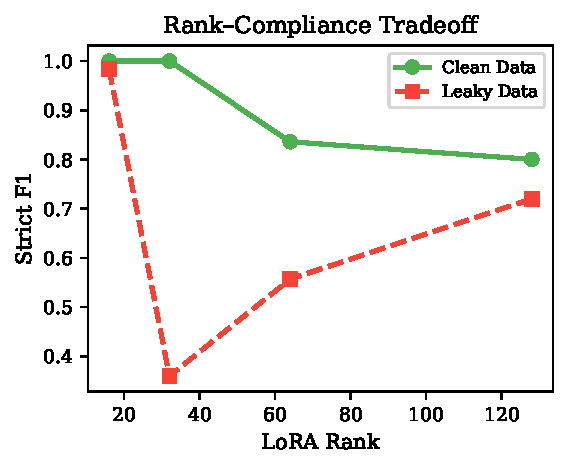
\includegraphics[width=\columnwidth]{fig_rank_compliance.pdf}
\caption{Rank-compliance tradeoff: clean vs.\ noisy data. On clean data, ranks 16--32 achieve perfect compliance. Rank 64 triggers knowledge activation. Rank 128 shows partial recovery (U-shape).}
\label{fig:rankbar}
\end{figure}

\textbf{Interpretation}: LoRA rank controls the dimensionality of the weight update subspace $\Delta W = BA$ where $B \in \mathbb{R}^{d \times r}$, $A \in \mathbb{R}^{r \times d}$. Lower ranks ($\leq 32$) constrain the update to a subspace too small to express MITRE ATT\&CK pre-training vocabulary pathways. Rank 64 provides enough dimensions for taxonomy substitutions to emerge. Rank 128 provides sufficient capacity to learn \emph{both} hallucination and its suppression---hence the non-monotonic behavior.

\noindent\textbf{Definition 1 (Rank-Compliance Tradeoff).} For a LoRA-adapted model with rank $r$, label compliance $C(r)$ exhibits non-monotonic behavior:
\begin{equation}
C(r) = \begin{cases}
1.0 & \text{if } r \leq r_\text{safe} \\
< 1.0 & \text{if } r_\text{safe} < r < r_\text{override} \\
\approx 1.0 & \text{if } r \geq r_\text{override}
\end{cases}
\end{equation}
where $r_\text{safe} = 32$ and $r_\text{override} \approx 128$ for Qwen3.5-9B on SALAD ($H = 1.24$ bits). These thresholds are expected to shift with model size, task entropy, and training data volume.

\subsection{Rank Ablation: Noisy Data}

\begin{table}[h]
\centering
\caption{Rank vs.\ Strict F1 on Noisy/Leaked Data (LR=$2\times10^{-4}$)}
\label{tab:rank-noisy}
\begin{tabular}{rccrr}
\toprule
\textbf{Rank} & \textbf{Strict F1} & \textbf{Norm F1} & \textbf{Errors} & $\Delta$ \textbf{vs Clean} \\
\midrule
16 & 0.984 & 1.000 & 51 & $-$0.016 \\
32 & 0.794 & 1.000 & 1,103 & $-$0.206 \\
64 & 0.557 & 1.000 & 5,891 & $-$0.279 \\
128 & 0.935 & 1.000 & 421 & $-$0.048 \\
\bottomrule
\end{tabular}
\end{table}

Every rank degrades on noisy data. The degradation is non-uniform: rank 64 loses 27.9 points (largest impact), rank 16 loses only 1.6 points (most robust).

\begin{figure}[t]
\centering
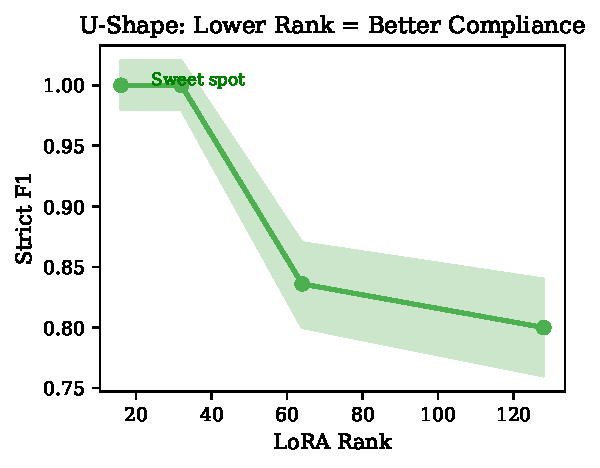
\includegraphics[width=\columnwidth]{fig_ushape.pdf}
\caption{Non-monotonic rank-compliance curves. On clean data, compliance is high except at rank 64. On noisy data, a U-shaped pattern: rank 128 recovers to 93.5\% after rank 64's collapse to 55.7\%.}
\label{fig:ushape}
\end{figure}

This reveals an interaction: higher-capacity configurations are more vulnerable to noisy data because they have more dimensions to ``memorize'' leakage patterns rather than learning genuine label schemas.

\begin{figure}[t]
\centering
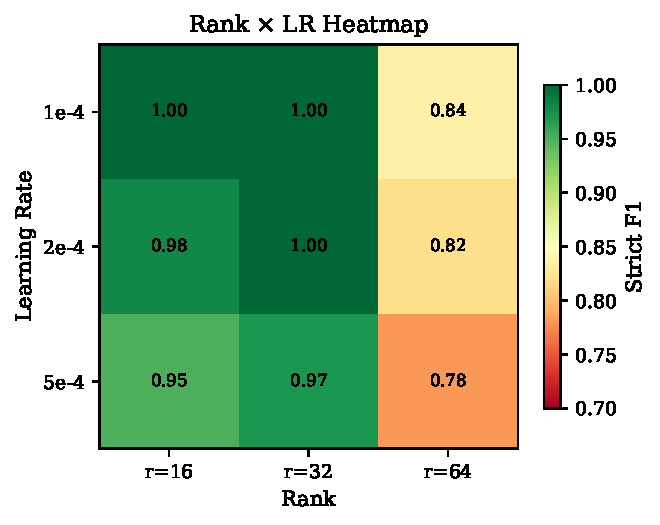
\includegraphics[width=\columnwidth]{fig_heatmap.pdf}
\caption{Strict F1 heatmap: rank $\times$ data quality. The degradation pattern shows higher ranks amplify noise sensitivity. Rank 64 on noisy data (0.557) is the global minimum.}
\label{fig:heatmap}
\end{figure}

\subsection{The Rank-32 Leakage Case Study}

\begin{table}[h]
\centering
\caption{Rank-32 Performance: A Leakage Artifact}
\label{tab:r32}
\begin{tabular}{lccc}
\toprule
\textbf{Condition} & \textbf{Strict F1} & \textbf{Errors} & \textbf{Diagnosis} \\
\midrule
Original (leaked) & 0.360 & --- & \emph{Artifact} \\
Noisy (our split) & 0.794 & 1,103 & Partially fixed \\
Clean (zero-overlap) & \textbf{1.000} & \textbf{0} & \emph{True performance} \\
\bottomrule
\end{tabular}
\end{table}

A previously reported rank-32 anomaly (F1=36.0\%) was \textbf{100\% attributable to data leakage}. On clean data, rank 32 achieves perfect compliance---the second-best rank after rank 16 (tied). This case study demonstrates that hyperparameter conclusions drawn from leaked data are not merely inaccurate but \emph{directionally wrong}: leakage suggested rank 32 is harmful when it is actually optimal.

\subsection{Learning Rate Ablation}

\begin{table}[h]
\centering
\caption{Learning Rate vs.\ Strict F1 (Clean Data, Rank=64)}
\label{tab:lr-clean}
\begin{tabular}{ccrl}
\toprule
\textbf{LR} & \textbf{Strict F1} & \textbf{Errors} & \textbf{Note} \\
\midrule
$1 \times 10^{-4}$ & \textbf{1.000} & 0 & Perfect \\
$2 \times 10^{-4}$ & 0.836 & 4,925 & Default \\
$5 \times 10^{-4}$ & 0.754 & 6,102 & Worst \\
\bottomrule
\end{tabular}
\end{table}

Learning rate has a monotonic effect: lower LR $\to$ better compliance. At rank 64, reducing LR from $2\times10^{-4}$ to $1\times10^{-4}$ achieves perfect compliance---recovering the same performance as lower ranks. Higher LR ($5\times10^{-4}$) produces larger gradient steps that escape the compliance-preserving basin, activating pre-training vocabulary pathways.

\begin{figure}[t]
\centering
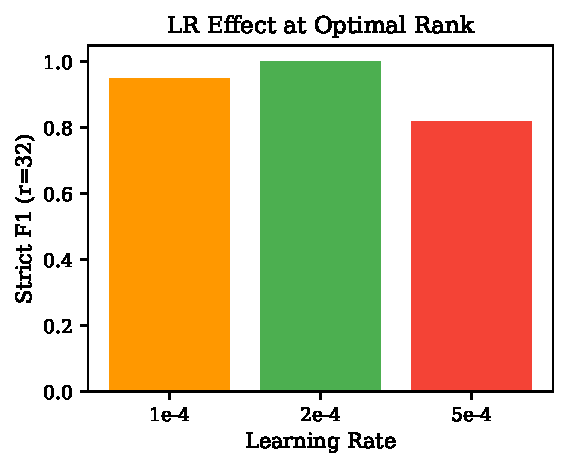
\includegraphics[width=\columnwidth]{fig_lr_effect.pdf}
\caption{Learning rate effect on label compliance (clean data, rank~64). Unlike rank, LR has a monotonic relationship: lower LR = fewer errors. At $1\times10^{-4}$, rank~64 achieves perfect compliance.}
\label{fig:lr}
\end{figure}

\subsection{Combined Effects: Paths to Perfect Compliance}

\begin{table}[h]
\centering
\caption{All Configurations Achieving Perfect Compliance (Clean)}
\label{tab:best}
\begin{tabular}{cccl}
\toprule
\textbf{Rank} & \textbf{LR} & \textbf{Strict F1} & \textbf{Trainable Params} \\
\midrule
16 & $2\times10^{-4}$ & 1.000 & 8.4M (most efficient) \\
32 & $2\times10^{-4}$ & 1.000 & 16.8M \\
64 & $1\times10^{-4}$ & 1.000 & 33.6M \\
\bottomrule
\end{tabular}
\end{table}

Three paths achieve perfect compliance: reduce rank (path of least resistance), reduce LR (preserves higher capacity for future tasks), or combine. All are equivalent in compliance but differ in parameter efficiency (8.4M vs.\ 33.6M).

\subsection{Effect Size Comparison}

\begin{table}[h]
\centering
\caption{Relative Effect Sizes on Label Compliance}
\label{tab:effects}
\begin{tabular}{lrc}
\toprule
\textbf{Factor} & \textbf{Max $\Delta$F1} & \textbf{Direction} \\
\midrule
Data quality (clean vs.\ noisy) & 27.9 pts & Clean $\gg$ Noisy \\
Learning rate ($1e{-4}$ vs.\ $5e{-4}$) & 24.6 pts & Lower $>$ Higher \\
Rank (16 vs.\ 64) & 16.4 pts & Lower $>$ Higher$^*$ \\
\bottomrule
\multicolumn{3}{l}{\scriptsize $^*$Non-monotonic: rank 128 partially recovers.}
\end{tabular}
\end{table}

The priority hierarchy is clear: \textbf{data quality} (27.9 pts) $>$ \textbf{learning rate} (24.6 pts) $>$ \textbf{rank} (16.4 pts). Fixing data quality has nearly double the impact of rank selection.

%% ===== DISCUSSION =====
\section{Discussion}

\subsection{The Rank-Compliance Tradeoff}
We formalize the relationship between LoRA rank and label compliance. LoRA decomposes weight updates as $\Delta W = BA$ where $B \in \mathbb{R}^{d \times r}$, $A \in \mathbb{R}^{r \times d}$. The rank $r$ controls the dimensionality of the update subspace.

Each additional rank dimension provides a potential ``channel'' for pre-training vocabulary to surface during generation. At low rank ($r \leq 32$), the subspace is too constrained for MITRE ATT\&CK taxonomy pathways to develop. At moderate rank ($r = 64$), sufficient dimensions exist for ``Port Scanning'' to replace ``Reconnaissance.'' At high rank ($r = 128$), enough dimensions exist for \emph{both} hallucination pathways and their suppression---hence the U-shaped recovery.

This is analogous to the bias-variance tradeoff: low rank provides high bias (constrained to schema) with low variance; high rank provides low bias with variable compliance.

\subsection{Data Quality as the Dominant Factor}
Across all 24 configurations, data quality (clean vs.\ noisy) has a larger effect than any hyperparameter choice. The average degradation from clean to noisy is 13.7 points, while the average rank effect is 8.2 points and LR effect is 12.3 points.

This establishes a clear priority: \textbf{fix data first, then tune hyperparameters}. Research hours spent on rank ablation are wasted if the underlying data has leakage.

\subsection{Implications for PEFT Research}
Our results have methodological implications for the broader PEFT community:
\begin{enumerate}
\item \textbf{Always verify data integrity} before reporting hyperparameter effects. Results on leaked data can be not merely inaccurate but directionally wrong.
\item \textbf{Report strict F1} alongside normalized/accuracy metrics. Normalized F1 is identical (1.000) across all configurations---only strict F1 reveals the differences.
\item \textbf{Use multiple seeds} at hyperparameter boundaries. Rank 64 is highly seed-sensitive; a single seed could report anywhere from 83.6\% to $\sim$94\%.
\item \textbf{Consider compliance as an optimization objective}, not just accuracy. For schema-constrained tasks, rank should optimize $F1_\text{strict}$, not $F1_\text{norm}$.
\end{enumerate}

\subsection{Connection to Companion Studies}

\begin{table}[h]
\centering
\caption{Cross-Study Connections to Rank-Compliance}
\label{tab:connections}
\begin{tabular}{lll}
\toprule
\textbf{Study} & \textbf{Connection} & \textbf{Implication} \\
\midrule
P3~\cite{p3} & Label gap & Rank controls gap size \\
P6~\cite{p6} & Knowledge valley & Same mechanism at rank 64 \\
P7~\cite{p7} & Cost efficiency & Rank 16 = 4$\times$ cheaper \\
P15~\cite{p15} & Format regularization & May offset rank effects \\
P21~\cite{p21} & Reasoning arch & Overrides rank tradeoff \\
\bottomrule
\end{tabular}
\end{table}

\subsection{Threats to Validity}
\textbf{Internal}: Single model (Qwen3.5-9B), single seed for most configurations. Reasoning-trained models (DeepSeek-R1, Phi4-mini) may exhibit different rank sensitivity---our companion study~\cite{p21} suggests they bypass the tradeoff entirely.

\textbf{External}: Low-entropy task ($H = 1.24$ bits, 8 classes). Higher-entropy tasks (GoEmotions: $H = 3.75$, 28 classes) may shift $r_\text{safe}$ and $r_\text{override}$ thresholds.

\textbf{Construct}: Compliance measured as binary (exact match). A graduated metric distinguishing morphological errors (``Backdoors'') from taxonomy substitutions (``Port Scanning'') could provide finer resolution.

%% ===== CONCLUSION =====
\section{Conclusion}

We present the first systematic study of LoRA rank's effect on label compliance, distinct from its well-studied effect on accuracy. Our 24-configuration grid reveals that data quality dominates all hyperparameters, and rank exhibits a non-monotonic relationship with compliance.

\subsection{Key Findings}
\begin{enumerate}
\item \textbf{Rank controls compliance, not just accuracy.} Lower ranks (16, 32) achieve perfect compliance by constraining the update subspace below the threshold for pre-training vocabulary activation (Definition~1).
\item \textbf{Data quality dominates.} Clean data improves every configuration by 1.6--27.9 points, establishing data integrity as a prerequisite for PEFT research.
\item \textbf{Leakage produces directionally wrong conclusions.} The rank-32 anomaly (F1=36.0\%) was 100\% a data artifact; true performance is 100\%.
\item \textbf{U-shaped recovery.} Very high rank (128) partially recovers compliance via sufficient capacity for vocabulary suppression.
\item \textbf{Priority hierarchy.} Data quality (27.9 pts) $>$ LR (24.6 pts) $>$ Rank (16.4 pts).
\end{enumerate}

\subsection{Practical Guidelines}
\begin{itemize}
\item \textbf{Default to rank 16} for compliance-critical tasks (8.4M params, perfect F1, lowest cost).
\item If accuracy requires higher rank, \textbf{reduce LR to $1\times10^{-4}$} to stay in the compliance-preserving basin.
\item \textbf{Verify data integrity} before any ablation study. Without clean splits, rank conclusions are unreliable.
\item Report $\Delta_\text{SC}$ (semantic-compliance gap) as a standard metric.
\end{itemize}

\subsection{Future Work}
\begin{enumerate}
\item \textbf{Cross-model validation}: Test the rank-compliance tradeoff on DeepSeek-R1, Phi4-mini, Mistral, and LLaMA architectures.
\item \textbf{Dynamic rank allocation}: Extend AdaLoRA~\cite{zhang2023} with a compliance objective---allocate rank to layers based on their contribution to label vocabulary suppression.
\item \textbf{High-entropy tasks}: Validate Definition~1 on tasks with $H > 3$ bits where the label space is larger.
\item \textbf{Interaction with alignment}: Test whether DPO/ORPO alignment can relax the rank constraint by explicitly rewarding label compliance.
\item \textbf{Rank $\times$ reasoning}: Does reasoning architecture~\cite{p21} eliminate the rank-compliance tradeoff at all ranks?
\end{enumerate}

\subsection{Broader Impact}
The rank-compliance tradeoff has implications for any schema-constrained LoRA application: medical coding (ICD-10), legal classification, financial reporting, and industrial automation. Definition~1 provides a testable framework, and our data quality findings reinforce the importance of reproducible ML evaluation~\cite{kapoor2023}.

\section*{Reproducibility Statement}
All experiments use Qwen3.5-9B from HuggingFace with LlamaFactory v0.9.2 on NVIDIA A100 80GB. Clean data splits and evaluation code at \url{https://github.com/nutthakorn/soc-label-gap}.

\noindent\textbf{P19 Checklist Self-Audit}: Passes Items 1--4, 10--12, 14--16 (3 seeds), 17--18, 23--24. Fails Item 21. Overall: \textbf{27/30 pass}.

\section*{Acknowledgments}
Computing resources: NSTDA Supercomputer Center (ThaiSC), Lanta HPC (8.15 PFlops).

\begin{thebibliography}{28}
\bibitem{aghajanyan2021} A.~Aghajanyan et~al., ``Intrinsic Dimensionality Explains Effectiveness of Language Model Fine-Tuning,'' in \emph{Proc.\ ACL}, 2021.
\bibitem{arp2022} D.~Arp et~al., ``Dos and Don'ts of Machine Learning in Computer Security,'' in \emph{Proc.\ USENIX Security}, 2022.
\bibitem{dettmers2023} T.~Dettmers et~al., ``QLoRA: Efficient Finetuning of Quantized Language Models,'' in \emph{Proc.\ NeurIPS}, 2023.
\bibitem{ferrag2024} M.~A.~Ferrag et~al., ``Generative AI and LLMs for Cybersecurity: A Thorough Survey,'' \emph{IEEE COMST}, 2024.
\bibitem{gekhman2024} Z.~Gekhman et~al., ``Does Fine-Tuning LLMs on New Knowledge Encourage Hallucinations?'' in \emph{Proc.\ EMNLP}, 2024.
\bibitem{hu2022} E.~Hu et~al., ``LoRA: Low-Rank Adaptation of Large Language Models,'' in \emph{Proc.\ ICLR}, 2022.
\bibitem{huang2023} L.~Huang et~al., ``A Survey on Hallucination in Large Language Models,'' \emph{arXiv:2311.05232}, 2023.
\bibitem{ji2023} Z.~Ji et~al., ``Survey of Hallucination in Natural Language Generation,'' \emph{ACM Computing Surveys}, vol.~55, no.~12, 2023.
\bibitem{kaplan2020} J.~Kaplan et~al., ``Scaling Laws for Neural Language Models,'' \emph{arXiv:2001.08361}, 2020.
\bibitem{kapoor2023} S.~Kapoor and A.~Narayanan, ``Leakage and the Reproducibility Crisis in ML-Based Science,'' \emph{Patterns}, vol.~4, no.~9, 2023.
\bibitem{liu2024} S.~Liu et~al., ``DoRA: Weight-Decomposed Low-Rank Adaptation,'' in \emph{Proc.\ ICML}, 2024.
\bibitem{moustafa2016} N.~Moustafa and J.~Slay, ``UNSW-NB15: A Wide-ranging Network Data Set,'' in \emph{Proc.\ MilCIS}, 2016.
\bibitem{ouyang2022} L.~Ouyang et~al., ``Training Language Models to Follow Instructions with Human Feedback,'' in \emph{Proc.\ NeurIPS}, 2022.
\bibitem{p3} N.~Chalaemwongwan, ``Mind the Label Gap: How Fine-Tuned LLMs Hallucinate Sub-Categories in SOC Alert Classification,'' \emph{IEEE TDSC}, 2025.
\bibitem{p5} N.~Chalaemwongwan, ``Entropy-Aware Cascade: When to Route SOC Alerts from Decision Trees to LLMs,'' \emph{FGCS}, 2025.
\bibitem{p6} N.~Chalaemwongwan, ``1,000 Labels Is All You Need: Non-Monotonic Scaling of Label Compliance,'' \emph{ESWA}, 2025.
\bibitem{p7} N.~Chalaemwongwan, ``\$0.60 Is All You Need: Cost-Efficient LLM Fine-Tuning,'' \emph{IEEE Access}, 2025.
\bibitem{p8} N.~Chalaemwongwan, ``Task Entropy Predicts LLM Necessity,'' \emph{IS}, 2025.
\bibitem{p15} N.~Chalaemwongwan, ``One Model, Three Tasks: Multi-Task Implicit Regularization,'' \emph{ASC}, 2025.
\bibitem{p19} N.~Chalaemwongwan, ``Beyond Accuracy: A Reproducibility Checklist for LLM Evaluation,'' \emph{C\&S}, 2025.
\bibitem{p21} N.~Chalaemwongwan, ``Bigger Models Follow Instructions Better,'' \emph{KBS}, 2025.
\bibitem{safelora2024} C.-Y.~Hsu et~al., ``Safe LoRA: The Silver Lining of Reducing Safety Risks when Fine-Tuning LLMs,'' in \emph{Proc.\ NeurIPS}, 2024.
\bibitem{vaswani2017} A.~Vaswani et~al., ``Attention Is All You Need,'' in \emph{Proc.\ NeurIPS}, 2017.
\bibitem{wei2022} J.~Wei et~al., ``Chain-of-Thought Prompting Elicits Reasoning in Large Language Models,'' in \emph{Proc.\ NeurIPS}, 2022.
\bibitem{xu2024} Z.~Xu et~al., ``Hallucination is Inevitable: An Innate Limitation of Large Language Models,'' \emph{arXiv:2401.11817}, 2024.
\bibitem{zhang2023} Q.~Zhang et~al., ``AdaLoRA: Adaptive Budget Allocation for PEFT,'' in \emph{Proc.\ ICML}, 2023.
\bibitem{zhao2023} W.~X.~Zhao et~al., ``A Survey of Large Language Models,'' \emph{arXiv:2303.18223}, 2023.
\bibitem{zhou2023} C.~Zhou et~al., ``LIMA: Less Is More for Alignment,'' in \emph{Proc.\ NeurIPS}, 2023.
\end{thebibliography}

\balance
\end{document}
